%%%%%%%%%%%%%%%%%%%%%%%%%%%%%%%%%%%%%%%%%
% Dreuw & Deselaer's Poster
% LaTeX Template
% Version 2.0 (February 18, 2023)
%
% This template originates from:
% https://www.LaTeXTemplates.com
%
% Authors:
% Vel (vel@latextemplates.com)
% Philippe Dreuw and Thomas Deselaers (https://github.com/deselaers/latex-beamerposter)
%
% License:
% CC BY-NC-SA 4.0 (https://creativecommons.org/licenses/by-nc-sa/4.0/)
%
% NOTE: The bibliography needs to be compiled using the bibtex engine.
%
%%%%%%%%%%%%%%%%%%%%%%%%%%%%%%%%%%%%%%%%%

%----------------------------------------------------------------------------------------
%	PACKAGES AND OTHER DOCUMENT CONFIGURATIONS
%----------------------------------------------------------------------------------------

\documentclass{beamer} % Use the beamer base class

\usepackage[
	orientation=portrait, % Portrait orientation
	size=a1, % Paper size
	scale=1.5, % Scale, it's important to adjust this so your content fits nicely in the template
]{beamerposter} % Use the beamerposter package to create the layout

\usetheme{I6pd2} % Use the I6pd2 theme supplied with this template

\usepackage{changepage} % Required for temporarily indenting text blocks

\usepackage{amsmath,amsthm,amssymb,latexsym} % For including math equations, theorems, symbols, etc
\usepackage{physics}
\usepackage{gfsdidot} % Use the GFS Didot font

\usepackage{booktabs} % Top and bottom rules for tables

\usefonttheme{professionalfonts}
%\usefonttheme[onlymath]{structureitalicserif} % Uses Computer Modern for maths

\graphicspath{{Figures/}} % Location of figure images

%----------------------------------------------------------------------------------------
%	TITLE SECTION
%----------------------------------------------------------------------------------------

\title{\LARGE Can disease spread be modelled by a reaction-diffusion equation?} % Poster title

\author{Oliver Clift\textsuperscript{1}, James Emberton\textsuperscript{1}, Isaac Millen\textsuperscript{1}, Nicholas Mitchiner\textsuperscript{1}, Edward Phillips\textsuperscript{1} and Dominik Szablonski\textsuperscript{1}} % Author(s)

\institute{\textsuperscript{1}Department of Physics, University of Manchester} % Institution(s)

%----------------------------------------------------------------------------------------
%	FOOTER TEXT
%----------------------------------------------------------------------------------------

\newcommand{\leftfoot}{} % Left footer text

\newcommand{\rightfoot}{} % Right footer text

%\setbeamertemplate{footline}{} % Uncomment this line to hide the footer

%----------------------------------------------------------------------------------------

\begin{document}
	
\begin{frame}[t] % The whole poster is enclosed in one beamer frame, the [t] parameter aligns everything to the top

\begin{columns}[t] % Begin multi-column layout, the [t] parameter aligns each column's content to the top

\begin{column}{0.02\textwidth}\end{column} % Empty column for horizontal whitespace

\end{columns}

\hspace{0.015\textwidth}%
\begin{minipage}{0.97\textwidth}
\begin{block}{Abstract}
	In this study, we modelled the spread of disease in Manchester through a reaction-diffusion equation, comparing this to pre-lockdown Covid data. The main assumptions of the model were a constant population density, a recovery time of 14 days, and effects on immunocompromised people is ignored. The Euler method is used to solve the equation computationally. Our study successfully/unsuccessfully modelled spatial disease spread when comparing to pre-pandemic Covid data, but only the initial spread. The model could be improved by implementing random-walks to model more random behaviour, modelling more outbreak centres, or accounting for disease spread reduction.
\end{block}
\end{minipage}

\begin{columns}[t]
\begin{column}{0.02\textwidth}\end{column}

\begin{column}{0.465\textwidth} % Start the first content column


%----------------------------------------------------------------------------------------
%	INTRODUCTION
%----------------------------------------------------------------------------------------
            
\begin{block}{Introduction}
	Modelling disease spread is important for governments have appropriate plans in case of large-scale pandemics. The recent Covid pandemic was not handled very well (give some examples, probably cite some things here). With this motivation, we attempted to model the disease spread within greater Manchester. Using our knowledge of physics, we supposed that the spread of a disease like Covid could be modelled by a diffusion equation.
	
	\bigskip
	
	However, due to mass conservation, a standard diffusion equation is incapable of accurately modelling disease spread, because diseases are inherently create new infections. Therefore, for disease modelling, a reaction-diffusion equation is much so that the number of infections at any time is not conserved. This allows us to model new infections and patient recovery.
\end{block}

%----------------------------------------------------------------------------------------
%	MATERIALS
%----------------------------------------------------------------------------------------

\begin{block}{Theory - Reaction-Diffusion Equation} 
	We attempt to model the spread of disease via a reaction-diffusion equation,
	\begin{equation}
		\pdv{I}{t} = D\grad^2I + \beta(x,y)SI 	- \gamma I,
	\end{equation}
	which models spatial densities $\rho$, which are parametrised such that,
	\begin{equation}
		\rho = S + I + R,
	\end{equation}
	where,
	\begin{itemize}
		\item $S(x,y,t)$: Susceptible population.
		\begin{itemize}
			\item Those who can catch disease.
		\end{itemize}
		\item $I(x,y,t)$: Infected population.
		\begin{itemize}
			\item Those who have the disease.
		\end{itemize}
		\item $R(x,y,t)$: Recovered population.
		\begin{itemize}
			\item Those who are no longer infected.
		\end{itemize}
	\end{itemize}
\end{block}

%----------------------------------------------------------------------------------------

\end{column} % End of the first column

\begin{column}{0.03\textwidth}\end{column} % Empty column for horizontal whitespace
 
\begin{column}{0.465\textwidth} % Start the second content column

%----------------------------------------------------------------------------------------
%	RESULTS
%----------------------------------------------------------------------------------------

\begin{block}{Results: Simulation vs Data}
	Put things here
\end{block}

%------------------------------------------------

\begin{block}{Results: Figures}
	\begin{figure}
		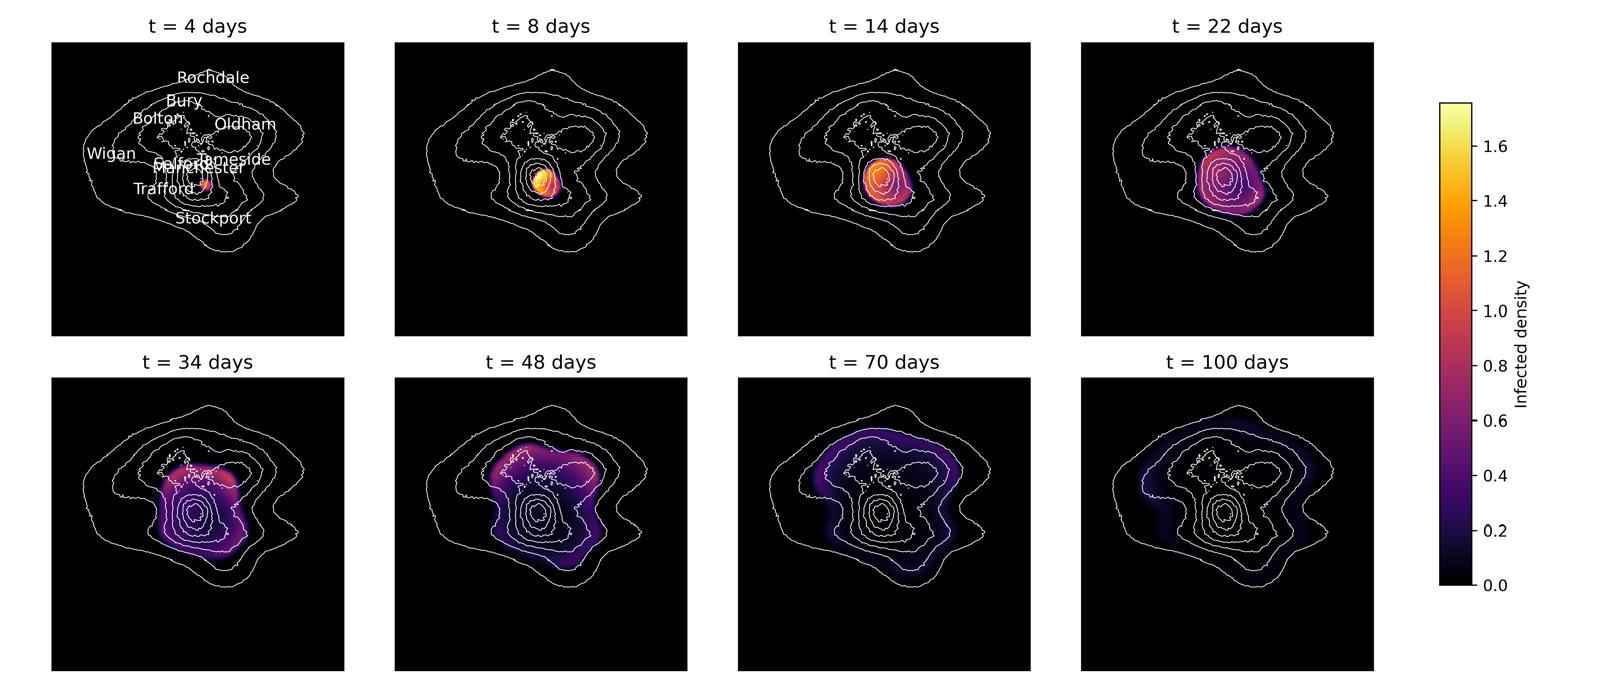
\includegraphics[width=\linewidth]{time.jpg}
		\caption{Disease spreading over time in Greater Manchester.}
	\end{figure}
\end{block}

\begin{block}{Discussion}
	We compared our model's output to that of the Covid pandemic. We founf that though our model was successful at modelling the initial spread of the infection, our results started to diverge as time went on. This is likely due to the assumption made that infected people do not change their behaviour when infected. This isn't true in real life, as infected people started to self isolate, and the country went into lockdown in March of 2020. This is a limitation of the model, but suggests that the model would be successful in modelling the behaviour of a pandemic should there be no outside intervention.
\end{block}

%----------------------------------------------------------------------------------------
%	CONCLUSIONS
%----------------------------------------------------------------------------------------

\begin{block}{Conclusions}
	We things out ig. 
\end{block}

%----------------------------------------------------------------------------------------
%	REFERENCES
%----------------------------------------------------------------------------------------

\begin{block}{References}
	\nocite{*} % Insert publications even if they are not cited in the poster
	\small % Reduce font size
	\vspace{-1ex} % Pull up slightly
	\bibliographystyle{unsrt} % Bibliography style
	\bibliography{sample.bib} % Bibliography file
\end{block}


%----------------------------------------------------------------------------------------

\end{column} % End of the second column

\begin{column}{0.02\textwidth}\end{column} % Empty column for horizontal whitespace

\end{columns} % End of all the columns in the poster

\end{frame} % End of the enclosing frame

%----------------------------------------------------------------------------------------

\end{document}
